\documentclass[12pt,fleqn]{article}\usepackage{../../common}
\begin{document}
Simulasyon

�nce basit bir sim�lasyon kodlayal�m. Fiziksel parametreleri ��yle, yer�ekimi
sabiti $g$ 0.8 (d�nyadan daha az), toplar�n birbirine ya da duvara �arpmas�
sonucu hi� enerji kayb� olmuyor. Grafik y�ntemi �urada [1] i�lendi. Toplar�n
birbirine �arpma sonucu h�z vekt�rlerinin hesab� [4]'te. 

\inputminted[fontsize=\footnotesize]{python}{sim1.py}

Kodda yak�nl�k i�in b�le� kullan�ld� [3].

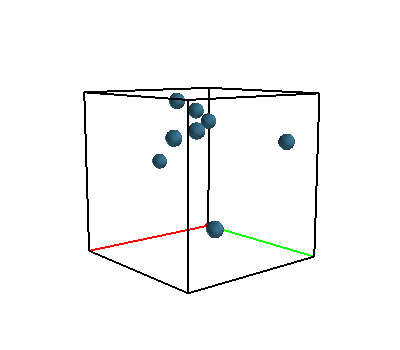
\includegraphics[width=15em]{glutout-140.png}
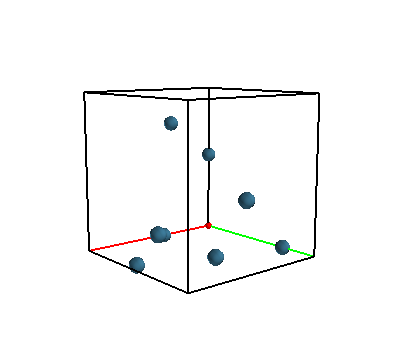
\includegraphics[width=15em]{glutout-390.png}

T�m resimleri birle�tirirsek,

\begin{minted}[fontsize=\footnotesize]{python}
convert -scale 30% /tmp/glutout-*.png /tmp/balls1.gif
\end{minted}

Sonu� [2]'de g�r�lebilir.


Kaynaklar

[1] Bayramli, {\em OpenGL, PyOpenGL}, \url{https://burakbayramli.github.io/dersblog/sk/2020/08/pyopengl.html}

[2] Bayramli, {\em Simulasyon 1 Animasyon},
    \url{https://github.com/burakbayramli/classnotes/blob/master/phy/phy_007_sim/balls1.gif?raw=true}

[3] Bayramli, Bilgisayar Bilim, {\em En Yak�n k-Kom�u (k-Nearest Neighbor), Geometrik Yak�nl�k Hesab�} 

[4] Bayramli, Fizik, {\em Temel Fizik 2, D�n��ler, Bas�n�, �arp��ma}


\end{document}
